\documentclass[final,onefignum,onetabnum]{siamart190516}
\usepackage[utf8]{inputenc}
\usepackage{geometry, graphicx,wrapfig}
\usepackage{enumerate}
\usepackage{amsmath,amssymb,amsfonts,bm}%,amsthm}
\usepackage{xcolor} %just for visible comments.
\usepackage[linesnumbered,ruled,vlined,algo2e]{algorithm2e}
\usepackage[toc,page]{appendix}
\usepackage{makecell}
\usepackage{cleveref}
\usepackage{pdfpages}

% New theorems and commands
\newtheorem{assump}[theorem]{MP Setting}
\newcommand\mycommfont[1]{\ttfamily\textcolor{orange}{#1}}
\newcommand{\R}{\mathbb{R}}
\newcommand{\F}{\mathbb{F}}
\newcommand{\dd}{\delta}
\newcommand{\tth}{\theta}
\newcommand{\bb}[1]{\mathbf{#1}}
\newcommand{\fl}{\mathrm{fl}}
\newcommand{\cO}{\mathcal{O}}
\newcommand{\red}[1]{\textcolor{red}{#1}}
\begin{document}
\title{Response to Reviewers}
\date{}
\maketitle
We are grateful to our editor, Laura Grigori, for handling the reviews of our paper, and to both reviewers for their constructive criticisms.

Our response to the reviews is below, and we have appended a diff file at the end that highlights which changes have been made.\\

\noindent{\bf Reviewer \#1}
In my opinion, the manuscript is still in need of major revision. 
Please note that line numbers here correspond to those in the diff file.
\begin{enumerate}
	\item I still have some issue with the lack of assumptions on $u^{(h)}$ vs. $u^{(l)}$ in the ``ad hoc'' setting. I still don't see how you can get around needing $u^{(h)} \lesssim (u^{(l)})^2$, as otherwise you can not guarantee "exact" products as you do in your proof in lines 167-172 and thus you cannot ignore errors from computing the products as you do in (2.8). \\
	In your response you said ``However, we are trying to leave the analysis general so that other combinations of floating point numbers can be considered as well'', but there is nothing general about the proof in lines 167-172.  Also, in lines 165-166, you say here that the exact products in MP Setting 2.3 are done by using fp16 as low precision and fp32 as high precision. So is that the case (in which case the value of the disparity in precisions is clear), or are you trying to be more general (in which case I still think you need h to be at least double the precision of l)? I do not think that the assumption $u^{(h)} \lesssim (u^{(l)})^2$ will limit you technically, since this is actually the case in TensoreCore bFMAs.
	
	\item Another major point is that looking at the plots in Figure 2, I am curious how uniform precision methods in fp16 would do compared to the "mp*2" variants. In other words, is there any benefit at all to doing "mp*2" variants, or would it be just as good numerically to do the whole thing in fp16?
	
	\item Another general comment is that it seems like a large amount of text is devoted to comparing accuracy of and bounds for TSQR vs. HQR, but I'm not sure this comparison is very meaningful; the differences seem very minor (as evidenced in Figure 2).
	
	\item {\it line 17: These are not my areas of expertise, but I did not think that QR factorization was used in any of the mentioned applications (clustering, ranking graph algorithms, neural network training). It therefore sounds strange to say that the investigation of mixed precision QR is a "first step" towards mixed precision implementations of such applications.}\\
	\red{ Not sure how to reply to this. }
	
	\item {\it line 40-41: I still disagree with the way this sentence is written, which makes it sound like no mixed precision analyses exist. There are certainly mixed precision analyses of linear algebra routines, dating back to the 60s. You could change the sentence to something like ``Many existing rounding error analyses ...''}\\
	{\bf Done.}
	
	\item {\it line 191: In (2.8), the summation upper limit should be $m$ instead of $n$.}\\
	{\bf Done.}
	
	\item {\it lines 241: ``swept into'' rather than ``swept under''; remove the word ``assumption''}\\
	{\bf Done.}
	
	\item {\it line 242: ``Using these two mixed precision settings''. Which two? I only see one ``MP Setting''}.\\
	{\bf Clarified.}
	
	\item {\it line 248: ``analyzed the inner product in an ad hoc mixed precision inner product''. Should it be ``... ad hoc mixed precision setting''?}\\
	{\bf Done.}
	
	\item {\it line 249: Don't need to spell out the HH acronym again, this is already done earlier. Actually, there is a bit of a confusion here. Earlier, e.g., line 46, Householder QR is abbreviated as ``HH QR'', but then in Section 3 Householder QR is abbreviated ``HQR''. }\\
	{\bf We will abbreviate Householder as HH for all instances except for the standard Householder QR algorithm, which we'll abbreviate as HQR.}
	
	\item {\it lines 298-299: Again, ``swept under our use'' sounds strange in this context. I would instead say ``swept that minor difference into the constant defined in the $\tilde{\gamma}$ notation ...''.}\\
	{\bf Done.}
	
	\item {\it lines 305-306 and 308: ``At iteration" $\rightarrow$ ``In iteration" }\\
	{\bf Done.}
	
	\item {\it Lemma 3.2: I still don't understand where the ``n'' in the final product is coming from. Ditto in line 351.} \\
	{\bf Fixed.}
	
	
	\item {\it line 352: ``have 2-norm, 1'' $\rightarrow$ ``have unit 2-norm''}\\
	{\bf Done.}
	
	\item {\it Algorithm 4: Capitalize "householder" in caption.}\\
	{\bf Done.}
	
	\item {\it line 395:  Remove comma after "matrix".}\\
	{\bf Done.}
	
	\item {\it line 407:  Use ``bFMA'' acronym already defined. }\\
	{\bf Done.}
	
	\item {\it line 409:  ``negligible" appears twice? Also, ``does not" $\rightarrow$ ``do not"}\\
	{\bf Done.}	
	
	\item {\it line 412: ``result a" $\rightarrow$ ``result in a"}\\
	{\bf Done.}
	
	\item{\it line 417: ``consist of" $\rightarrow$ ``consists of"; spacing after ``1)" and ``2)".}\\
	{\bf Done.}
	
	\item {\it line 419: Consider changing ``exact variant" to ``particular variant" to avoid any confusion. Also, change ``denote ... to be the outputs" to ``let ... denote the outputs".}\\
	{\bf Done.}
	
	\item {\it line 430: ``$(k-1)r+1^{st}$" $\rightarrow$ ``$((k-1)r+1)^{th}$", ``$kr^{th}$" $\rightarrow$ ``$(kr)^{th}$". Or better yet, reword to "... corresponds to columns (k-1)r+1 through kr of ..."}\\
	{\bf Done.}
	
	\item {\it line 489: ``outperform" $\rightarrow$ "achieve higher accuracy than" ?}\\
	{\bf Done.}
	
	\item {\it Section 3.3: Include some definition of what ``Tall and skinny" means? (Doesn't come until line 509)}\\
	{\bf Added.}
	
	\item {\it line 504: Why are there parentheses around L in ``$2^{(L)}$"?}\\
	{\bf Removed parentheses.}
	
	\item {\it line 517: Capitalize beginning of sentence.}\\
	{\bf Done.}
	
	\item {\it line 529: Should "$2^{(\ell)}$" be "$2^L$" here? Ditto 2x in the following line. }\\
	{\bf Yes.}
	
	\item {\it line 538: Remove comma after "matrix".}\\
	{\bf Removed.}
	
	\item {\it line 564: "stability is not guaranteed in HQR"..."the method is stable when using TQSR". This needs a more careful definition of what you mean by "stability". HQR is indeed normwise backward stable (we know this from a result of Wilkinson), and indeed, your example here obeys the known bounds on the normwise relative backward error if you plug in the parameters you used. It is not that the method isn't backward stable, it is simply that the choice of parameters here means that the computed quantites are not very good. }\\
	\red{ Not sure how to reply to this. }
	
	
	\item {\it line 565: Clarify this sentence. Something like "Note that these worst-case bounds are likely overestimates in practice".}\\
	{\bf Done.}
	
	\item {\it Figure 1: Make font bigger. Also, in the last paragraph in Section 3, you should maybe comment on the bounds on $\Delta Q$, since this is what is shown in the figure (rather than the relative backward error). }\\
	{\bf }
	
	\item line 656: "casted up" $\rightarrow$ "cast up"
	
	\item line 657: "casted down" $\rightarrow$ "cast down"
	
	\item line 662: "Since $\hat{W}_k$, $\hat{Y}_k$'s are computed with alg. 4 in high precision then cast down" $\rightarrow$ "Since the $\hat{W}_k$, $\hat{Y}_k$'s in alg. 4 are computed in high precision and then cast down"
	
	\item line 663: "to some matrix stored in low precision, B" $\rightarrow$ "to some matrix B stored in low precision"
	
	\item Algorithm 7 caption: "of low precision A" $\rightarrow$ "on low precision A"
	
	\item line 679: ", we result in" $\rightarrow$ " results in"
	
	\item line 626: The latest A100 GPUs are not restricted to fp16/fp32 in the TensorCore instructions, which should be mentioned.
	
	\item lines 830: "varying size" $\rightarrow$ "varying matrix size"
	
	\item Figure 2: Font needs to be much bigger. What does the "h" mean here in the uniform precision setting, e.g., what is "HQRh" in the legend? The "h" in the label makes me think it is HQR in half precision, but the text says that the uniform precision is single. 
	
	
	\item Figure 3: I am very confused as to why the condition number has any effect. Overall, it is entirely unclear what the right plots are showing. What do the colors mean, and what does each line represent? What are the horizontal red lines? I would recommend just omitting this. 
	
\end{enumerate}
\noindent{\bf Reviewer \#1}
The authors have satisfactorily responded to all my comments and suggestions. I
recommend the paper to be accepted and provide a few more comments and suggestions
that do not require another review round.
\begin{enumerate}
	\item L61-63: the sentence defining the backward error that has been added is not so easy to understand , for clarity I would explicitly add that in the context of this paper the backward error is defined as $\|A- \hat{Q}\hat{R}\|$. Regarding the other reviewer’s comment, while it is true that $\|A-Q\hat{R}\|$  may more commonly be called backward error, $\|A-\hat{Q}\hat{R}\|$ is certainly also a valid definition.
	\item L388–389: negligible is repeated
	\item L388, 392, 653: compared to $\rightarrow$ compared with
	\item L635–636: this sentence refers to a result from subsection 4.2 which comes after. I would move this comment to subsection 4.2.
	\item L650–657: again, this would be better placed after section 4.2.
	\item Table 5: I suggest adding in the caption the definition of every variable: $m$, $n$, $N$, etc. The objective being to make this table self-contained for other articles to refer to it.
	\item Table 5, mpBQR2,3: be consistent in whether you factorize the $n^{1/2}$.
	\item L901: imporved (typo)
\end{enumerate}

\bibliographystyle{siamplain}%ieeetr
\bibliography{../../../../../library.bib,../../../../../sans_library.bib,./report.bib}

%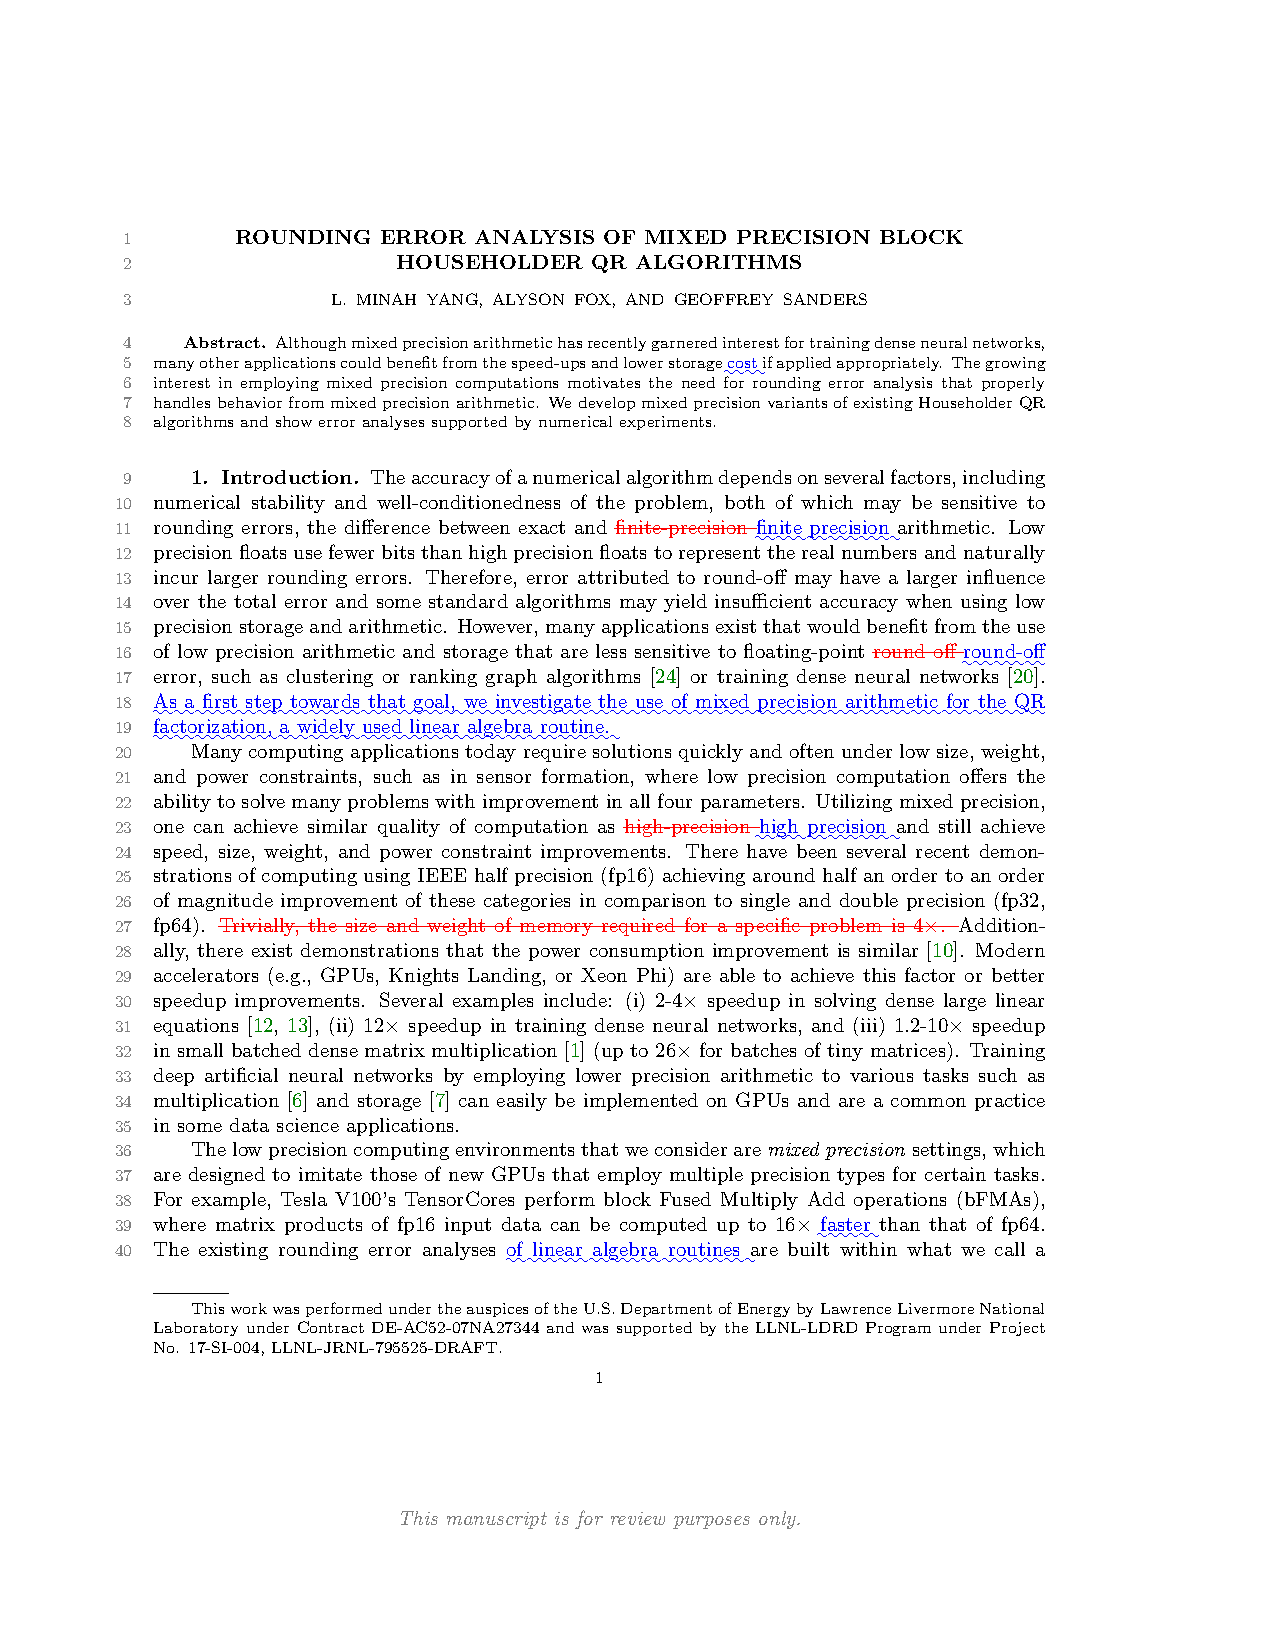
\includepdf[pages=-]{diff.pdf}
\end{document}